\documentclass[11pt, oneside]{article}    
\usepackage[margin=1in,letterpaper]{geometry}                     
\usepackage{times} 
\usepackage{graphicx}            
\usepackage{amssymb,amsmath}
\usepackage{array}
\usepackage[round]{natbib}
%\usepackage{hyperref}
\usepackage{color}
\usepackage[T1]{fontenc}
\usepackage{longtable}
\usepackage{wrapfig}
\usepackage{sectsty}
\sectionfont{\fontsize{12}{12}\selectfont}

%%%%%%%%%%%%%%%%%%%%%%%%%%%%%%%%%%%%%

\title{Electromagnetic wave propagation and interaction with matter}
\author{Brent Minchew}
%\date{}							% Activate to display a given date or no date

\begin{document}
\maketitle
%\thispagestyle{empty} %%% to remove page numbers
%\section{}
%\subsection{}

\section{Introduction}

%Our primary interest in these notes is in how EM waves interact with matter. Interactions involve combinations of scattering, absorption, transmission, and emission, each of which will be discussed in detail in due course. Here, we undertake a brief review of the salient properties of EM waves, their propagation in lossy and lossless media, and their reflection and transmission at planar boundaries. 

These notes offer a review of EM waves and are taken primarily from \citet{ulaby2014}, Chapter 2.

\section{Constitutive parameters}
\renewcommand\labelitemi{{\boldmath$\cdot$}}

The EM characteristics of any material can be described by four constitutive parameters:
\begin{enumerate}
	\item $\varepsilon'\varepsilon_0 $ is the electrical \emph{permittivity} 
	\begin{itemize}
		\item units: F/m, where F = Farad = J/V$^2$ is a unit of capacitance
		\item the measure of material's ability to store electrical energy in an electric field
		\item $\varepsilon_0 = 8.85\times10^{-12}$ F/m is the permittivity of free space (the minimum permittivity)
		\item $\varepsilon'$ is the permittivity of the material relative to the permittivity of free space; in general, we will only be interested in the relative permittivity $\varepsilon'$
		\item in all cases, $\varepsilon' \ge 1$ where unity applies only to free space
	\end{itemize}
	\item $\mu$ is the magnetic \emph{permeability} 
	\begin{itemize}
		\item units: H/m; H = Henry = J/A$^2$ is a unit of inductance
		\item the ability of a material to support the development of a magnetic field
		\item in all materials (except ferromagnetic materials), we can take $\mu = \mu_0$
		\item $\mu_0 = 4\pi\times10^{-7}$ H/m is the permeability of free space.
	\end{itemize}
	\item $\rho_v$ is the charge density 
	\begin{itemize}
	 	\item units: C/m$^3$; C = Coulomb = A$\cdot$s
		\item $\rho_v = 0$ in remote sensing applications and will not be considered in any detail in this course
	\end{itemize}
	\item $\sigma$ is the conductivity 
	\begin{itemize}
		\item units: S/m; S = Siemen = $\Omega^{-1}$ = A/V
		\item measure of a material's ability to allow current to flow through it
		\item analogous to inverse of resistance (note the units)
		\item accounts for power loss in a material, thus is of fundamental importance in remote sensing
		\item general categories and examples
			\begin{itemize}
				\item $\sigma = 0$ in a lossless material (free space)
				\item $\sigma \approx 0$ in low-loss materials (e.g., air)
				\item $\sigma > 0$ in lossy materials (e.g., salt water)
				\item $\sigma \gg 0$ in conductors (e.g., copper, gold, silver, etc.)
				\item $\sigma = \infty$ in perfect conductors
			\end{itemize}
	 \end{itemize}
\end{enumerate}

For remote sensing applications, we can simplify the above list by noting (later showing) that $\rho_v = 0$ for natural materials and that virtually all materials of interest in remote sensing applications have $\mu = \mu_0$. Further, we can define the (dimensionless) complex dielectric constant (sometimes called the complex permittivity or the relative dielectric constant)
	\begin{equation}
	\label{e:dielectric1}
	\varepsilon = \varepsilon' - j\varepsilon'' = \varepsilon' - j\frac{\sigma}{\omega \varepsilon_0}
	\end{equation}
where $j^2 = -1$, $\omega$ is the angular frequency of an EM wave (discussed later), and $\varepsilon''$ is the \emph{dielectric loss factor}\footnote{There are many other common ways to represent Eq. \ref{e:dielectric1}. Perhaps most common are the loss tangent $\tan{(\delta)} = \varepsilon''/\varepsilon'$ and the complex refractive index (or index of refraction) $n = \sqrt{\varepsilon}$, whose real component is $n' = c/\mathrm{v}_p$, where $c$ is the speed of light in a vacuum and $\mathrm{v}_p$ is the phase velocity of the EM wave.}. Eq. \ref{e:dielectric1} is one of the most important equations for this course. Note that nonzero conductivity implies attenuation (lossiness) through heating (e.g., microwave ovens operate on the principle that the water contained in food is conductive). Many remote sensing instruments have a narrow range of $\omega$, so the loss factor $\varepsilon''$ is usually a function of $\sigma$ of the medium. When taking a broader view of remote sensing, wherein $\omega$ varies by many orders of magnitude, it is important to recognize that both permittivity and conductivity are nontrivial functions of the frequency of the EM signal: $\varepsilon' = \varepsilon'(\omega)$ and $\sigma = \sigma(\omega)$. %This is one of the fundamental concepts of remote sensing. 

The dependence of permittivity and conductivity on the frequency of the EM radiation involves myriad mechanisms that contribute to scattering, absorption, and transmission. These mechanisms are key to understanding the information contained in remote sensing data, particularly in \emph{spectroscopy}. We undertake more detailed discussions  later in the course, but it is useful at this stage to give some examples and a broad classification of the three general types of mechanisms that govern the frequency dependence of permittivity and conductivity. First, geometric and physical optics can give rise to dispersive refraction (e.g., rainbows), scattering (e.g., blue sky), and reflection. Second, vibrational excitation of molecules and ions influence both permittivity and conductivity. Finally, electronic excitations can, for example, allow incident EM radiation to excite molecules to higher energy levels. These broad mechanisms provide some preliminary insight into the characteristics of Earth's atmospheric opacity as a function of EM wavelength (Fig. \ref{f:ematmo}). Frequency bands that are opaque primarily because of water vapor and oxygen absorption and are useful for remote sensing of the atmosphere. Transparent frequency bands are useful for terrestrial sensing and, of course, contain the visible-light portion of the EM spectrum. 



\begin{figure}[t]
\begin{center}
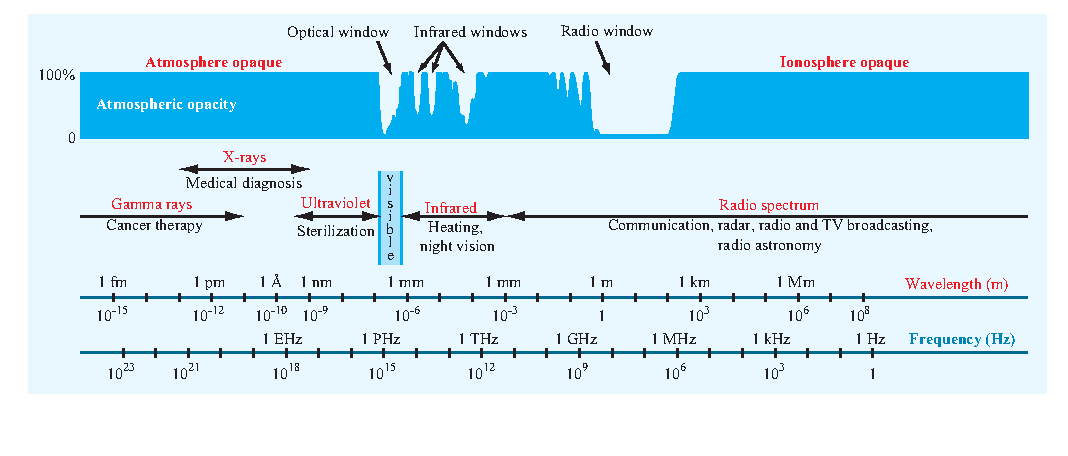
\includegraphics[width=\linewidth]{figs/em_atmosphere.pdf}
\caption{Atmospheric opacity for Earth (top) and the electromagnetic spectrum. Reproduced from \citep{ulaby2014}.}
\label{f:ematmo}
\end{center}
\end{figure}


\section{Maxwell's Equations}
In homogenous, isotropic media, we can write Maxwell's equations as
	\begin{subequations}
	\label{e:maxwell1}
	\begin{align}
	\nabla\cdot\mathbf{E} &= \frac{\rho_v}{\varepsilon'\varepsilon_0} \qquad\qquad\qquad\qquad \mathrm{Gauss's\ Law} \label{e:divE0} \\
	\nabla\cdot\mathbf{H} &= 0 \qquad\qquad\qquad\qquad\;\;\;\;\; \mathrm{Gauss's\ Law\ for\ magnetism}\\
	\nabla\times\mathbf{E} &= -\mu\frac{\partial \mathbf{H}}{\partial t} \qquad\qquad\qquad\;\;\; \mathrm{Faraday's\ Law} \label{e:curlE0} \\
	\nabla\times\mathbf{H} &= \varepsilon'\varepsilon_0\frac{\partial \mathbf{E}}{\partial t} + \sigma\mathbf{E}
			\qquad\qquad\ \mathrm{Amp\acute{e}re's\ Law} \label{e:curlH00}
	\end{align}
	\end{subequations}
where $\mathbf{E}$ and $\mathbf{H}$ are the electric (V/m) and magnetic (A/m) field intensities, respectively. Assuming the quantities $\mathbf{E}$ and $\mathbf{H}$ are phasors --- meaning that they are complex-valued, sinusoidal functions defined by their amplitude, angular frequency, and phase --- we can define the time-dependent electric field such that $\mathbf{E}(x,y,z,t) = \Re[\mathbf{E}(x,y,z)e^{j\omega t}]$ (similarly for the magnetic field). Amp\'ere's Law (Eq. \ref{e:curlH00}) can then be written
	\begin{equation}
	\label{e:curlH0}
	\begin{aligned}
	\nabla\times\mathbf{H} &= j\omega\varepsilon_0\left(\varepsilon' - j\frac{\sigma}{\omega\varepsilon_0}\right)\mathbf{E} \\
				&= j\omega\varepsilon\varepsilon_0\mathbf{E}
	\end{aligned}
	\end{equation}
where the dielectric constant $\varepsilon$ is defined in Eq. \ref{e:dielectric1}. Taking the divergence of Eq. \ref{e:curlH0} gives $\nabla\cdot\nabla\times\mathbf{H} \propto \nabla\cdot\mathbf{E}$. Recalling that the divergence of the curl of any vector is zero, we have $\nabla\cdot\mathbf{E} = 0$, requiring $\rho_v = 0$ from Gauss's Law (Eq. \ref{e:divE0}). Then, Maxwell's Equations (Eqs. \ref{e:maxwell1}) become
	\begin{subequations}
	\label{e:maxwell2}
	\begin{align}
	\nabla\cdot\mathbf{E} &= 0 \label{e:divE1} \\
	\nabla\cdot\mathbf{H} &= 0 \\
	\nabla\times\mathbf{E} &= -j\omega\mu \mathbf{H} \label{e:curlE1} \\
	\nabla\times\mathbf{H} &= j\omega\varepsilon\varepsilon_0\mathbf{E} \label{e:curlH1}
	\end{align}
	\end{subequations}
	
To derive the homogeneous wave equation\footnote{Why is Eq. \ref{e:waveeq1} a wave equation? To answer this, consider the simple case of a nonconducting material ($\sigma=0$), take the curl of Farraday's Law (Eq. \ref{e:curlE0}) and apply Amp\'{e}re's Law (Eq. \ref{e:curlH00}) and Gauss's Law (Eq. \ref{e:divE1}). Compare the resulting wave speed with the phase velocity defined in Eq. \ref{e:phasevel0}.} for the electric field, we can take the curl of Faraday's Law (Eq. \ref{e:curlE1}) and use Gauss's Law (Eq. \ref{e:divE1}) and Amp\'{e}re's Law (Eq. \ref{e:curlH1}) to get
	\begin{equation}
	\label{e:waveeq1}
	\nabla^2\mathbf{E} - \gamma^2\mathbf{E} = \mathbf{0}
	\end{equation}
where $\gamma$ is the complex-valued propagation constant\footnote{It is conventional in some fields to define a complex-valued angular wavenumber in place of a propagation constant (where the wavenumber would be equal to $-j\gamma$). As discussed later, we will define the wavenumber strictly as real-valued and equal to the angular frequency ($\omega$) divided by the phase velocity $\mathrm{v}_p$, as is common practice in remote sensing. } defined as
	\begin{equation}
	\gamma = j\omega\sqrt{\mu\varepsilon\varepsilon_0}
	\end{equation}
Similar steps can be taken for the magnetic field to get an expression identical to Eq. \ref{e:waveeq1} but with $\mathbf{H}$ in place of $\mathbf{E}$. As we shall see, the electric and magnetic fields can be related as
	\begin{subequations}
	\label{e:maxwell3}
	\begin{align}
	\mathbf{E} &=  -\eta\left(\hat{\mathbf{k}}\times\mathbf{H}\right) \\
	\mathbf{H} &= \hphantom{-} \frac{1}{\eta}\left( \hat{\mathbf{k}}\times\mathbf{E}\right)
	\end{align}
	\end{subequations}
where $\eta$ is the intrinsic impedance (defined later) and $\hat{\mathbf{k}}$ is the direction of travel of the EM wave. 

\section{Propagation of plane waves in lossless media}

A lossless medium is approximately lossless if $\varepsilon' \gg \varepsilon''$, so the relative dielectric constant is simply $\varepsilon \approx \varepsilon'$. In this case, the wavenumber can be defined as
	\begin{equation}
	\label{e:k1}
	k = \omega\sqrt{\mu\varepsilon'\varepsilon_0} = k_0\sqrt{\varepsilon'}
	\end{equation}
 and the wave equation (Eq. \ref{e:waveeq1}) becomes
 	\begin{equation}
	\label{e:waveeq2}
	\nabla^2\mathbf{E} + k^2\mathbf{E} = \mathbf{0}
	\end{equation} 
The wavenumber is the spatial analog of frequency and is related to the wavelength $\lambda$ as
	\begin{equation}
	k = \frac{2\pi}{\lambda}
	\end{equation}
and to the phase velocity $\mathrm{v}_p$ as\footnote{In a perfect vacuum, $\varepsilon' = 1$ and $\mu = \mu_0$, making $\mathrm{v}_p = c \approx 3\times10^8$ m/s, the speed of light in free space.}
	\begin{equation}
	\label{e:phasevel0}
	\mathrm{v}_p = \frac{\omega}{k} = \frac{1}{\sqrt{\mu_0\varepsilon'\varepsilon_0}} = \frac{c}{\sqrt{\varepsilon'}}
	\end{equation} 
where $c$ is the speed of light in a vacuum and the final two terms in Eq. \ref{e:phasevel0} are valid for nonmagnetic materials (\emph{i.e.,} virtually all materials of interest in remote sensing), for which $\mu=\mu_0$ is a reasonable approximation. In general, $\varepsilon' = \varepsilon'(\omega)$ and $\varepsilon' > 1$, so Eq. \ref{e:phasevel0} indicates that all materials are dispersive (to some extent) and that EM waves travel slower in the presence of matter relative to free space.

Now consider a uniform plane wave, in which the electric and magnetic fields have uniform properties at all points and the components of the electric and magnetic fields along the direction of propagation are zero. Let us define the plane wave in Cartesian coordinates as
	\begin{equation}
	\label{e:Efield_cart1} 
	\mathbf{E} = E_x\hat{\mathbf{x}} + E_y\hat{\mathbf{y}} + E_z\hat{\mathbf{z}}  
	\end{equation}
which gives
	\begin{equation}
	\label{e:Efield_cart2}
	\left(\frac{\partial^2}{\partial x^2} + \frac{\partial^2}{\partial y^2} + \frac{\partial^2}{\partial z^2} + k^2\right)E_i = 0
	\end{equation}
for $i = x,y,z$. For a wave propagating along $z$, the definition of a uniform plane wave requires $\partial E_x/\partial x = \partial E_x/\partial y = \partial E_y/\partial x = \partial E_y/\partial y = 0$ and $E_z = 0$ (and $H_z = 0$). Thus, Eq. \ref{e:Efield_cart2} reduces to
	\begin{equation}
	\label{e:Efield_cart3}
	\frac{\partial^2 E_x}{\partial z^2} + k^2E_x = 0 
	\end{equation}
with similar expressions for $E_y$ as well as the magnetic field components $H_x$ and $H_y$. The general solution to Eq. \ref{e:Efield_cart3} is
	\begin{equation}
	E_x(z) = E_{x0}^+e^{-jkz} + E_{x0}^-e^{jkz} 
	\end{equation}
where the first term on the righthand side indicates a wave with amplitude $E_{x0}^+$ traveling in the $+z$ direction. Likewise for the second term on the RHS. 

In the interest of simplicity, let us now orient our coordinate system such that $E_x$ is the only nonzero component of the electric field and consider only propagation in the $+z$ direction. Under these conditions, $\mathbf{E}(z) = E_{x0}^+e^{-jkz}\hat{\mathbf{x}}$. Now we solve for the associated magnetic field using Faraday's Law (Eq. \ref{e:curlE1}), whose only nonzero component is
	\begin{equation}
	H_y(z) = \frac{1}{\eta}E_{x0}^+e^{-jkz}
	\end{equation}
where
	\begin{equation}
	\eta = \frac{\omega\mu}{k} = \frac{\omega\mu}{\omega\sqrt{\mu\varepsilon'\varepsilon_0}} = \sqrt{\frac{\mu}{\varepsilon'\varepsilon_0}}
	\end{equation}
is the intrinsic impedance of a lossless medium\footnote{In a perfect vacuum, $\eta = \eta_0 = \sqrt{\mu_0/\varepsilon_0} \approx 377\ \Omega$, the intrinsic impedance of free space.}. 

In general, $E_{x0}^+$ will be complex, and defined in terms of a magnitude and phase $\phi^+$ as
	\begin{equation}
	E_{x0}^+ = |E_{x0}^+|e^{j\phi^+}
	\end{equation}
yielding instantaneous electric and magnetic fields defined as
	\begin{subequations}
	\label{e:EHphase1}
	\begin{align}
	\mathbf{E}(z,t) &= \left|E_{x0}^+\right|\cos\left(\omega t - kz + \phi^+\right)\hat{\mathbf{x}} \\
	\mathbf{H}(z,t) &= \frac{\left|E_{x0}^+\right|}{\eta}\cos\left(\omega t - kz + \phi^+\right)\hat{\mathbf{y}}
	\end{align}
	\end{subequations}
and shown for a specific case in Fig. \ref{f:EHspace}. From Eq. \ref{e:EHphase1} we can see that the electric and magnetic fields are in phase, a characteristic of lossless media. 

The approach taken in this section can be generalized to any uniform plane wave traveling in an arbitrary direction $\hat{\mathbf{k}}$, resulting in a relationship between $\mathbf{E}$ and $\mathbf{H}$ given in Eq. \ref{e:maxwell3} and repeated here for convenience
	\begin{subequations}
	\label{e:maxwell3a}
	\begin{align}
	\mathbf{E} &=  -\eta\left(\hat{\mathbf{k}}\times\mathbf{H}\right) \\
	\mathbf{H} &= \hphantom{-} \frac{1}{\eta}\left( \hat{\mathbf{k}}\times\mathbf{E}\right)
	\end{align}
	\end{subequations}
Note that these equations are valid for lossy media as well, so long as $\eta$ is appropriately defined. We will discuss the definition of $\eta$ for lossy media in later sections. 

\begin{figure}[t]
\begin{center}
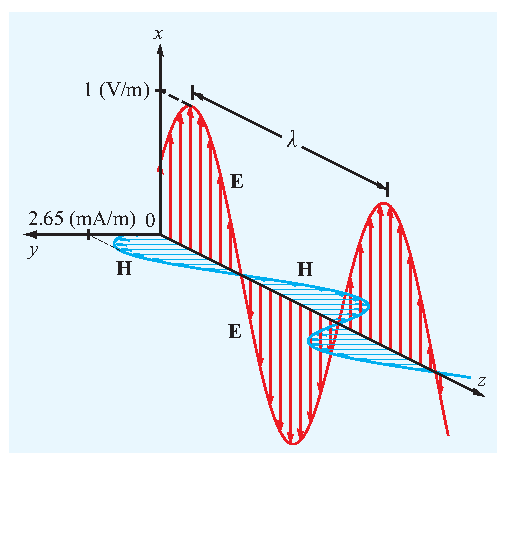
\includegraphics[width=8cm]{figs/em_wave_cartoon1.pdf}
\caption{Linearly polarized electric (red) and magnetic (blue) fields at $t=0$ propagating as uniform plane waves along $z$ with $\omega = 2\pi\times10^6$ rad/s, $k=2\pi/300$ rad/m, $\phi = \pi/3$, and $\eta = 1/2.65$. Note that the electric and magnetic fields are in phase (meaning their zero-crossings and, equivalently, their max values occur at the same $z$), indicating that these waves are in a lossless medium (\emph{i.e.,} $\eta$ is real-valued). In a lossy material, $\eta$ will be complex-valued (what we call $\eta_c$) and thereby will induce a phase shift between the electric and magnetic fields. Figure reproduced from \citep{ulaby2014}.}
\label{f:EHspace}
\end{center}
\end{figure}

\section{Wave polarization in a lossless medium}

In this section, we discuss the polarization of uniform plane waves, continuing to focus on lossless media for simplicity. The polarization of a uniform plane wave describes the path traced by the tip of the electric field vector over time at a given point in space. An ellipse is the most general path, but many remote sensing applications rely on the special cases of circular and linear polarizations; we will discuss each case. EM waves are not necessarily polarized (e.g., light from the sun is randomly polarized before passing through the atmosphere), but as we will see later in the course, the polarimetric properties of scattered EM waves can provide a wealth of information about the scatterer. 

Consider a uniform plane wave propagating in the $+z$ direction. From Eq. \ref{e:Efield_cart1} we have
	\begin{equation}
	\label{e:Efield_cart2aa} 
	\mathbf{E}(z) = E_x(z)\hat{\mathbf{x}} + E_y(z)\hat{\mathbf{y}}  
	\end{equation}
where the complex-valued amplitudes are
	\begin{subequations}
	\label{e:Efield_cart2a}
	\begin{align}
	E_x(z) &= E_{x0}e^{-jkz} = a_xe^{-j\left(kz-\delta_x\right)} \\
	E_y(z) &= E_{y0}e^{-jkz} = a_ye^{-j\left(kz-\delta_y\right)}
	\end{align}
	\end{subequations}
where $a_x = |E_{x0}|$ and $a_y = |E_{y0}|$ and $\delta_x$ and $\delta_y$ are the relative phases. The (real-valued) instantaneous electric field is then defined as
	\begin{equation}
	\label{e:Efield_cart3p}
	\mathbf{E}(z,t) = a_x\cos\left(\omega t - kz + \delta_x\right)\hat{\mathbf{x}} + 
					a_y\cos\left(\omega t - kz + \delta_y\right)\hat{\mathbf{y}}
	\end{equation}
Note that we do not need to specify the magnetic field because, based on the discussion above, they are uniquely defined by the electric field.

\begin{figure}[t]
\begin{center}
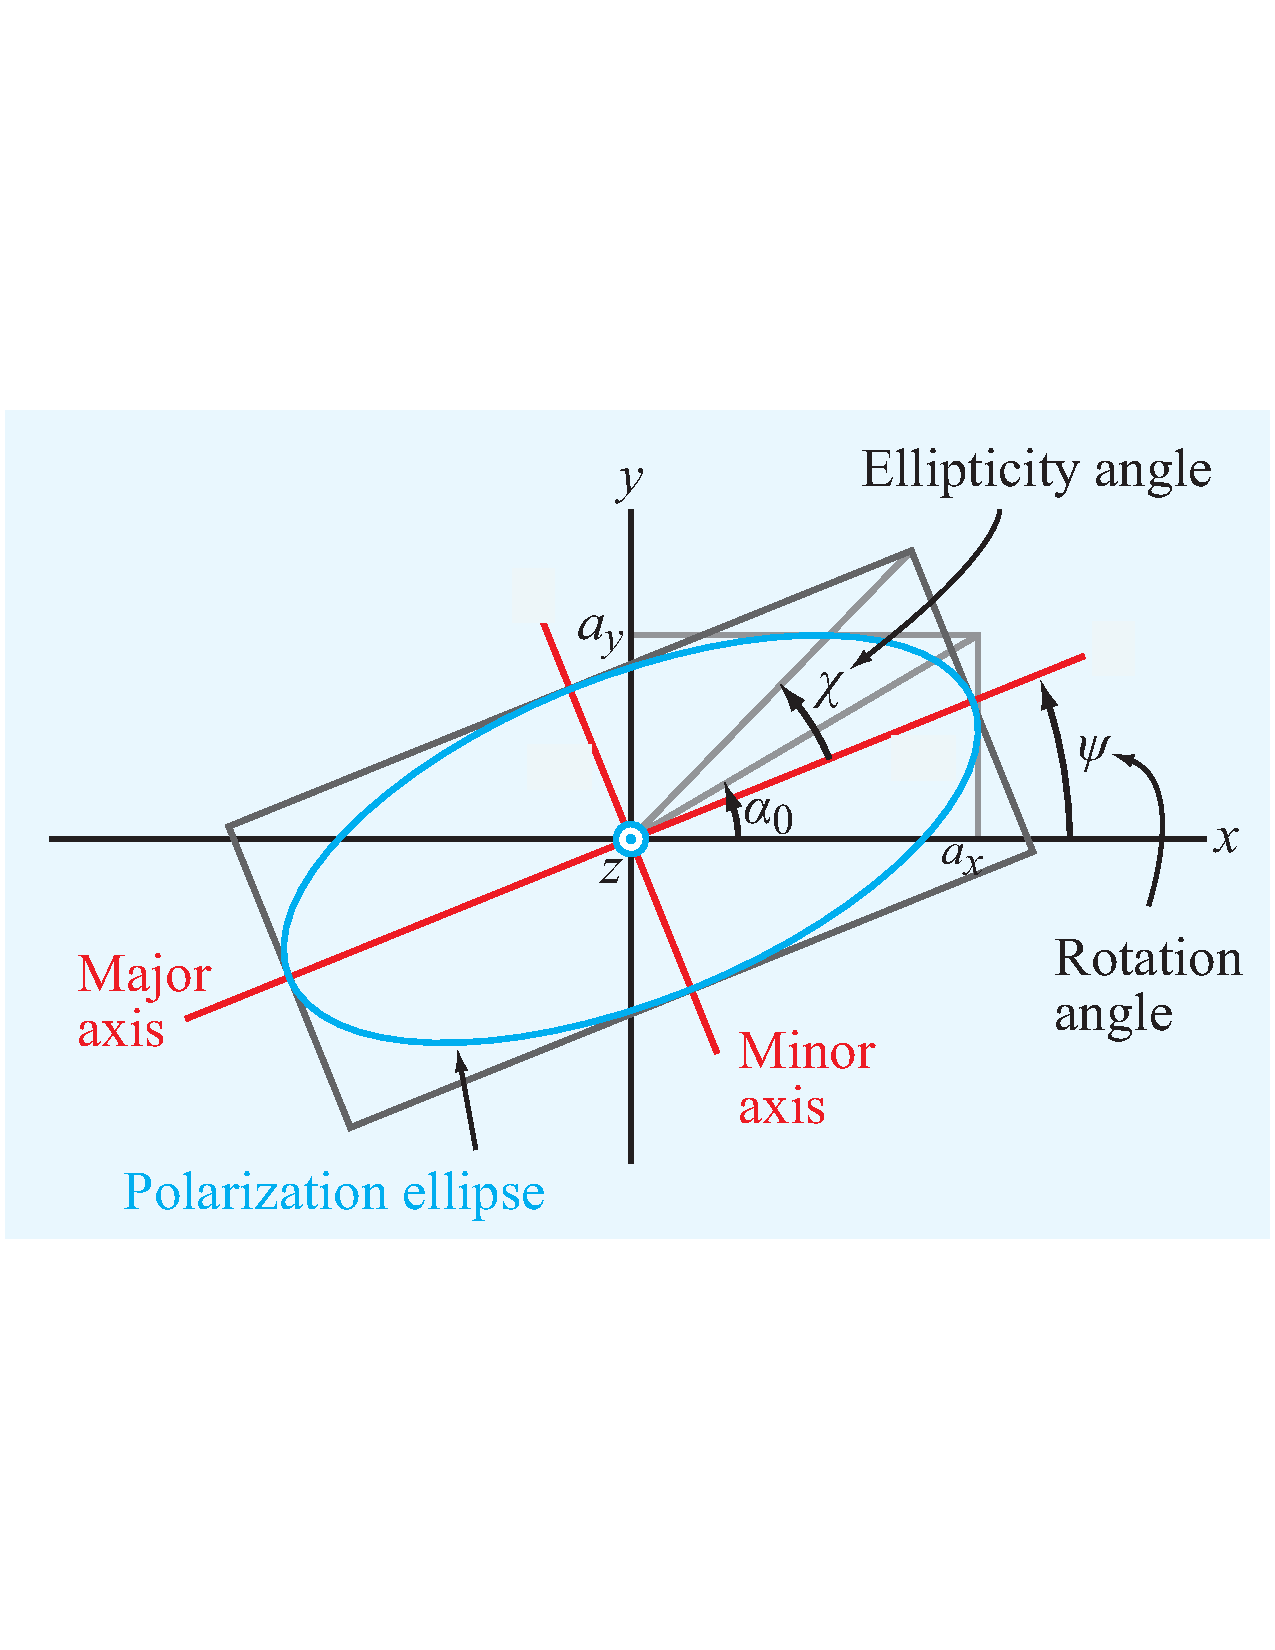
\includegraphics[width=10cm]{figs/em_polar_ellipse.pdf}
\caption{Polarization ellipse for a wave propagating out of the page. Modified from \citep{ulaby2014} }
\label{f:polellipse}
\end{center}
\end{figure}

Using Eq. \ref{e:Efield_cart3p}, it can be shown that the points on the locus of points traced by the tip of the electric field vector over time at a given spatial position satisfies the equation
	\begin{equation}
	\label{e:polarizationellipse}
	\left(\frac{E_x'}{a_x}\right)^2 + \left(\frac{E_y'}{a_y}\right)^2 - 
			2\frac{E_x'}{a_x}\frac{E_y'}{a_y}\cos{\delta} = \sin^2{\delta}
	\end{equation}
where $E_x' = \Re{[E_x]}$, $E_y' = \Re{[E_y]}$, and $\delta = \delta_y - \delta_x$. Eq. \ref{e:polarizationellipse} defines the polarization ellipse shown in Fig. \ref{f:polellipse}. The ellipse can be described by two angles --- the ellipse orientation angle $\psi$ ($0\le\psi\le\pi$) and the ellipticity angle $\chi$ ($-\pi/4 \le\chi\le\pi/4$) --- defined by the relations
	\begin{subequations}
	\label{e:polarizationellipse_angles}
	\begin{align}
	\tan{2\psi} &= \frac{2a_xa_y}{a_x^2-a_y^2}\cos{\delta} \\
	\sin{2\chi} &= \frac{2a_xa_y}{a_x^2+a_y^2}\sin{\delta}
	\end{align}
	\end{subequations}
and shown in Fig. \ref{f:polellipse}. The ellipse can be traced in either the clockwise or counterclockwise directions. Confusingly, the direction of rotation (\emph{i.e.}, the handedness) has two different conventions, depending on the frequency of the EM wave. For radar applications, the IEEE standard for handedness is defined as righthand (lefthand) polarization for electric fields rotating clockwise (counterclockwise) as seen by an observer watching the wave recede. For optical applications, standard convention is defined from the perspective of an observer seeing the wave approach. In other words, righthand polarization always corresponds to clockwise rotation and lefthand to counterclockwise; the difference between radar and optical is the whether the wave is going away (radar) or coming toward (optical) the observer. 

From Eqs. \ref{e:polarizationellipse} and \ref{e:polarizationellipse_angles}, it is straightforward to define the special cases of polarization often used in (active) remote sensing. The first is linear polarization, where $\delta = n\pi$ for any integer $n$ and $\chi = 0$. An example of a linearly polarized wave is shown in Fig. \ref{f:EHspace}. A circularly polarized wave occurs when $a_x = a_y$ and $\delta = \pm \pi/2$, where the sign denotes handedness. An example is showing in Fig. \ref{f:circpol}. Several examples of polarization states are shown in Fig. \ref{f:polstates}.

\begin{figure}[t]
\begin{center}
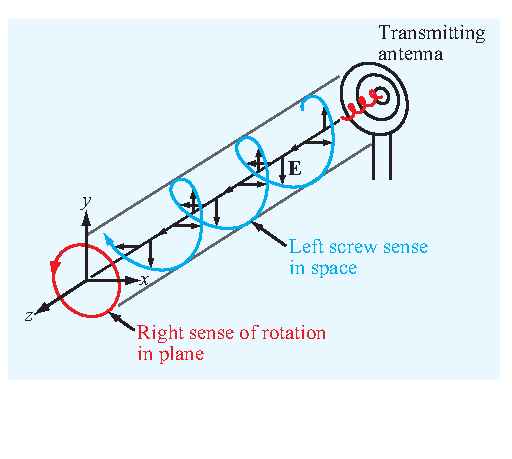
\includegraphics[width=10cm]{figs/em_polar_circular.pdf}
\caption{Righthand (radar convention) circularly polarized wave propagating in the $z$ direction. Reproduced from \citet{ulaby2014}.}
\label{f:circpol}
\end{center}
\end{figure}


\begin{figure}[t]
\begin{center}
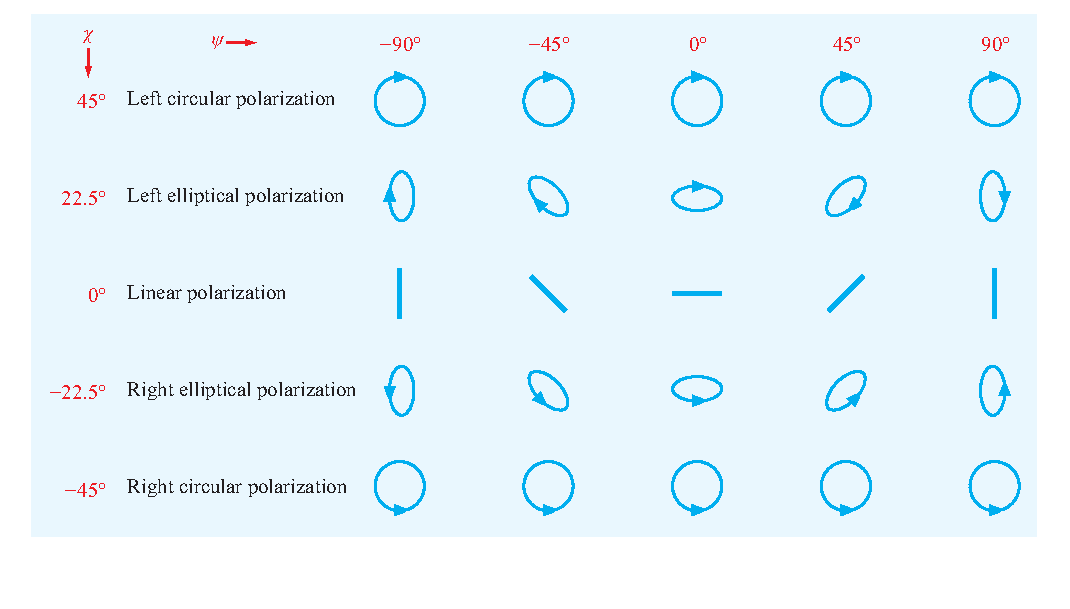
\includegraphics[width=\linewidth]{figs/em_polar_states.pdf}
\caption{Examples of polarization states for waves traveling out of the page. Handedness is given in radar convention. Reproduced from \citet{ulaby2014}.}
\label{f:polstates}
\end{center}
\end{figure}

There are numerous other methods for describing the polarization of a wave. Perhaps the most common is the Stokes vector (named after G. G. Stokes of Navier-Stokes-equations fame), whose components are defined as
	\begin{subequations}
	\label{e:stokes1}
	\begin{align}
	S_0 &= a_x^2 + a_y^2  \\
	S_1 &= a_x^2 - a_y^2 \\ %= S_0\cos{2\chi}\cos{2\psi} \\
	S_2 &= 2a_xa_y\cos\delta \\ %= S_0\cos{2\chi}\sin{2\psi} \\
	S_3 &= 2a_xa_y\sin\delta %= S_0\sin{2\chi}
	\end{align}
	\end{subequations}
Take a moment to compare the Stokes parameters with the terms in Eq. \ref{e:polarizationellipse_angles}. 

In fully polarized waves, $S_0$ is magnitude of the electric field and is related to the other Stokes parameters as
	\begin{equation}
	\label{e:S0}
	S_0^2 = S_1^2 + S_2^2 + S_3^2
	\end{equation}
Therefore, we can rewrite the three independent Stokes parameters as
	\begin{subequations}
	\label{e:stokes2}
	\begin{align}
	S_1 &= S_0\cos{2\chi}\cos{2\psi} \\
	S_2 &= S_0\cos{2\chi}\sin{2\psi} \\
	S_3 &= S_0\sin{2\chi}
	\end{align}
	\end{subequations}
which defines a sphere with radius $S_0$. This is known as the Poncar\'e sphere and is shown in Fig. \ref{f:poinsphere}. The Poncar\'e sphere is a useful tool for visualizing polarization states. All linear polarizations lie along the equator of the sphere ($\chi = 0$) while circular polarizations are found at the poles ($\chi = \pm \pi/2$). Orthogonal polarizations are antipodal on the Poncar\'e sphere. 


\begin{table}[h]
\caption{Common examples of Stokes vector}
\begin{center}
\begin{tabular}{c c c c l}
$S_0$ & $S_1$ & $S_2$ & $S_3$ & description \\  \hline
1 & 0 & 0 & 0 & randomly polarized \\
1 & 1 & 0 & 0 & linear, x-polarized \\
1 & -1 & 0 & 0 & linear, y-polarized \\
1 & 0 & 1 & 0 & linear, +45$^\circ$ \\
1 & 0 & -1 & 0 & linear, -45$^\circ$ \\
1 & 0 & 0 & 1 & righthand circular \\
1 & 0 & 0 & -1 & lefthand circular \\
\end{tabular}
\end{center}
\label{default}
\end{table}%


\begin{figure}[t]
\begin{center}
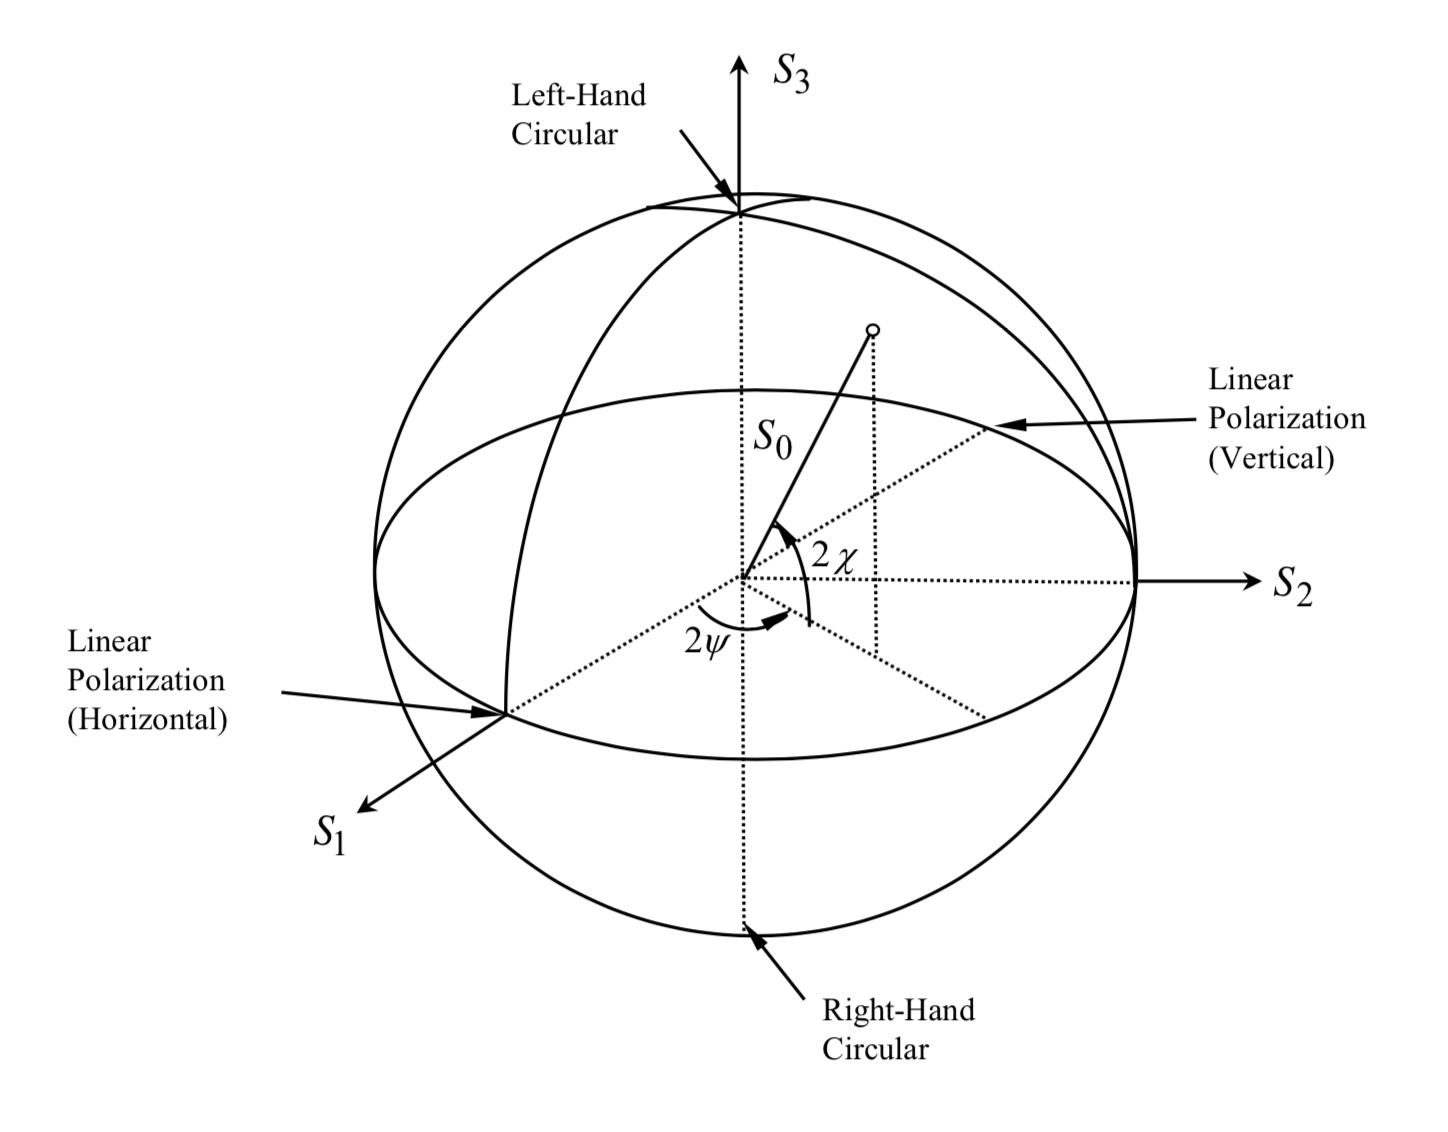
\includegraphics[width=12cm]{figs/poincare_sphere_vanzyl.png}
\caption{Poincar\'e sphere showing different polarization states. Handedness and linear polarization directions are given in radar convention. }
\label{f:poinsphere}
\end{center}
\end{figure}

In partially polarized waves, the Stokes parameters are related as
	\begin{equation}
	\label{e:S0u}
	S_0^2 \ge S_1^2 + S_2^2 + S_3^2
	\end{equation}
and the degree of polarization is defined as
	\begin{equation}
	\label{e:degpol}
	\mathcal{D} = \frac{\sqrt{S_1^2 + S_2^2 + S_3^2}}{S_0}
	\end{equation}
Equality in Eq. \ref{e:S0u} (and unity in Eq. \ref{e:degpol}) only holds for fully polarized waves. In the opposite extreme, the wave is unpolarized (or randomly polarized) and we have $S_0 > 0$ and $S_1=S_2=S_3 = 0$ (and $\mathcal{D} =0$). Finally, as a real-world and practical example, it is worth noting that an unpolarized wave can be defined as the sum of two fully polarized waves with orthogonal polarizations such that
	\begin{equation}
	\label{e:randpol}
	\left(\begin{array}{c} S_0 \\ 0\\ 0\\ 0\end{array}\right) = \frac{1}{2} \left(\begin{array}{c} S_0 \\ S_1\\ S_2\\ S_3\end{array}\right) +
			\frac{1}{2} \left(\begin{array}{r} S_0 \\ -S_1\\ -S_2\\ -S_3\end{array}\right)
	\end{equation}
Thus, when an unpolarized wave is incident on a polarized antenna (or sunglasses or some types of 3D movie glasses, etc.), the effective magnitude of the received wave is half that of the polarized wave. 

\section{Plane-wave propagation in lossy media}

\begin{figure}[t]
\begin{center}
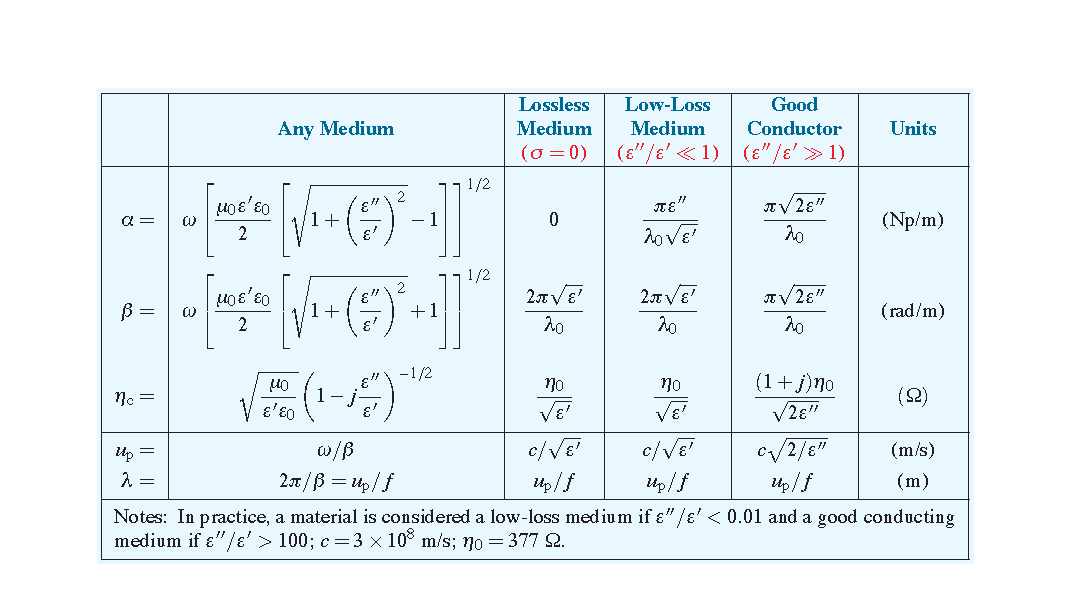
\includegraphics[width=\linewidth]{figs/em_lossy_table.pdf}
\caption{Summary table for the parameters of EM wave propagation in lossless and general lossy medium. For consistency, note that $k_0=2\pi/\lambda_0$, where $\lambda_0$ is the wavelength in free space, $f=\omega/(2\pi)$, and that $u_p\equiv \mathrm{v}_p = \omega/\beta$ is the phase velocity of the EM wave. Figure reproduced from \citet{ulaby2014}, Table 2-1.}
\label{f:emtable}
\end{center}
\end{figure}

Up to this point, we have focussed on lossless media. While this may be a good approximation in some cases (e.g., microwaves propagating through air), attenuation in many natural media may be important, and in some cases, the signal of interest. 

Let us start by recalling the EM wave equation in Eq. \ref{e:waveeq1}, in which the propagation constant is defined for a general medium as
	\begin{subequations}
	\label{e:gamma2}
	\begin{align}
	\gamma^2 &= -\omega^2\mu_0\varepsilon\varepsilon_0 \\
			&= -\omega^2\mu_0\varepsilon_0(\varepsilon' - j\varepsilon'') \\
			&= (\alpha + j\beta)^2
	\end{align}
	\end{subequations}
where the attenuation constant $\alpha$ and phase constant $\beta$ are defined as 
	\begin{subequations}
	\label{e:alphabeta1}
	\begin{align}
	\alpha &= -\omega \sqrt{\mu_0\varepsilon_0}\ \Im{\left\{\sqrt{\varepsilon}\right\}} \nonumber \\
		&= k_0\left\{ \frac{\varepsilon'}{2}\left[-1 + \sqrt{1+\left(\frac{\varepsilon''}{\varepsilon'}\right)^2} \right]\right\}^{1/2} \label{e:alpha1} \\ \nonumber \\ 
	\beta &= \omega\sqrt{\mu_0\varepsilon_0}\ \Re{\left\{\sqrt{\varepsilon}\right\}} \nonumber \\
		&= k_0\left\{ \frac{\varepsilon'}{2}\left[1 + \sqrt{1+\left(\frac{\varepsilon''}{\varepsilon'}\right)^2} \right]\right\}^{1/2} \label{e:beta1}
	\end{align}
	\end{subequations}
where $k_0 = 2\pi/\lambda_0$ is the (angular) wavenumber (and $\lambda_0$ is the wavelength) in free space\footnote{In this section and unless otherwise noted, we set $\mu = \mu_0$ because the virtually all materials of interest in remote sensing are nonmagnetic.}. Note that all terms inside the curly brackets are dimensionless. To gain some insight into as to how $\alpha$ and $\beta$ influence EM waves, consider the simple example of a uniform plane wave propagating along $z$ of the form of Eq. \ref{e:Efield_cart3}, but replacing $k$ with $\gamma$. Plugging in Eq. \ref{e:gamma2}, we get
	\begin{equation}
	\label{e:wave_e_alphabeta}
	\mathbf{E}(z) = \hat{\mathbf{x}}E_{x0}e^{-\gamma z} = \hat{\mathbf{x}}E_{x0}e^{-\alpha z}e^{-j\beta z}
	\end{equation}
and
	\begin{equation}
	\label{e:wave_h_alphabeta}
	\mathbf{H}(z) = \hat{\mathbf{y}}\frac{E_{x0}}{\eta_c}e^{-\alpha z}e^{-j\beta z}
	\end{equation}
where 
	\begin{equation}
	\label{e:eta_c}
	\eta_c = \frac{\eta_0}{\sqrt{\varepsilon'}}\left(1-j\frac{\varepsilon''}{\varepsilon'}\right)^{-1/2}
	\end{equation}
is the intrinsic impedance of a lossy material and $\eta_0 = \sqrt{\mu_0/\varepsilon_0}$ is the intrinsic impedance of free space. When the material is conductive (meaning $\varepsilon'' > 0$), $\eta_c$ is complex-valued, which results in a (constant) phase shift between the magnetic and electric fields. Because the phase of the electric field is governed by $\beta$, the phase velocity for an EM wave propagating in a general lossy medium is
	\begin{equation}
	\label{e:vp_lossy}
	\mathrm{v}_p = \frac{\omega}{\beta}
	\end{equation}
Compare Eq. \ref{e:vp_lossy} with Eq. \ref{e:phasevel0} and note conductivity reduces the phase velocity. 

\begin{figure}[t]
\begin{center}
\begin{tabular}{c c}
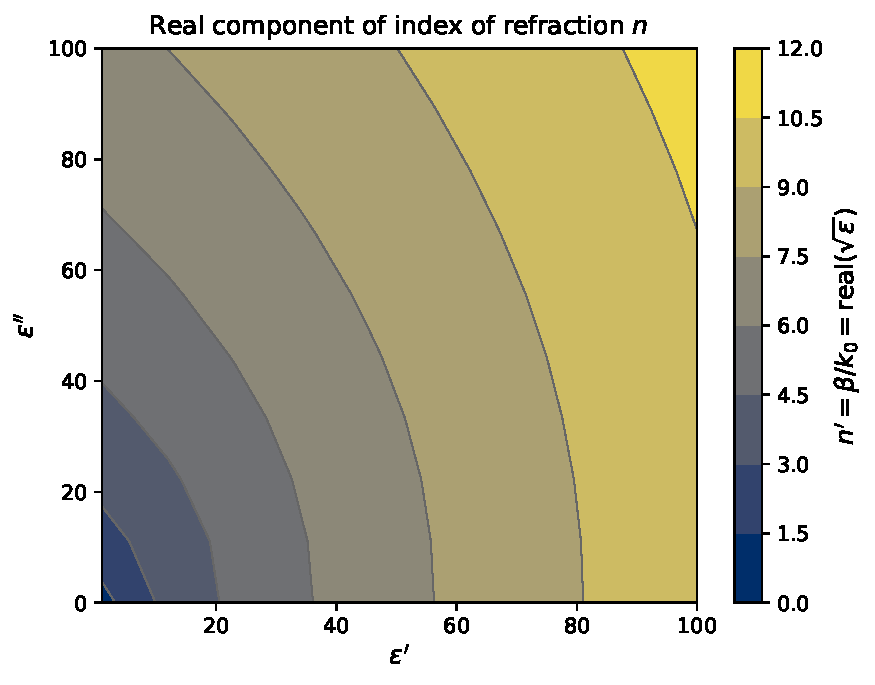
\includegraphics[height=6.6cm]{figs/refrac_index_real.pdf} & 
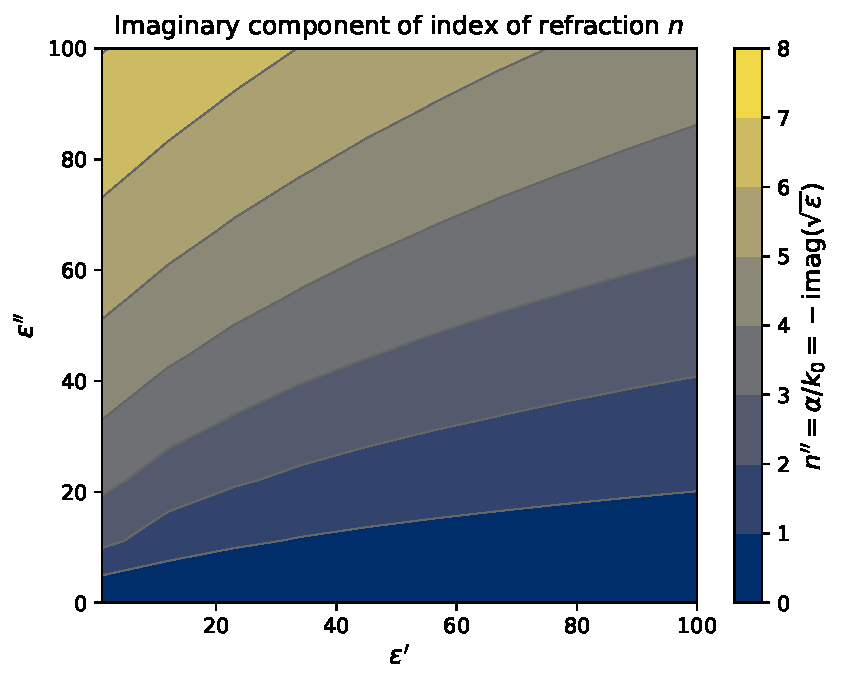
\includegraphics[height=6.6cm]{figs/refrac_index_imag.pdf}
\end{tabular}
\caption{Real (left) and imaginary (right) components of the complex index of refraction. These are equivalent to the phase and attenuation constants, $\alpha$ and $\beta$, normalized by the free-space wavenumber. }
\label{default}
\end{center}
\end{figure}


From Eq. \ref{e:wave_e_alphabeta}, we can see that nonzero $\alpha$ serves only to attenuate the EM signal while $\beta$ only influences the phase of the EM signal, consistent with their respective monikers. In some remote sensing applications, we are concerned with the depth to which the signal can penetrate. Eq. \ref{e:wave_e_alphabeta} indicates that the \emph{skin depth}, defined as the depth at which the magnitude of the electric field decreases by a factor of $1/e$, is given as
	\begin{equation}
	\label{e:skindepth}
	\delta_s = 1/\alpha
	\end{equation}
It is sometimes common to define a \emph{penetration depth} --- the depth at which the power of the electric field decreases by a factor of $1/e$ --- as $\delta_p = \delta_s/2$. As expected, $\delta_s \to \infty$ as $\alpha \to 0$, indicating that a plane wave can propagate indefinitely in a lossless medium. 

\begin{figure}[t]
\begin{center}
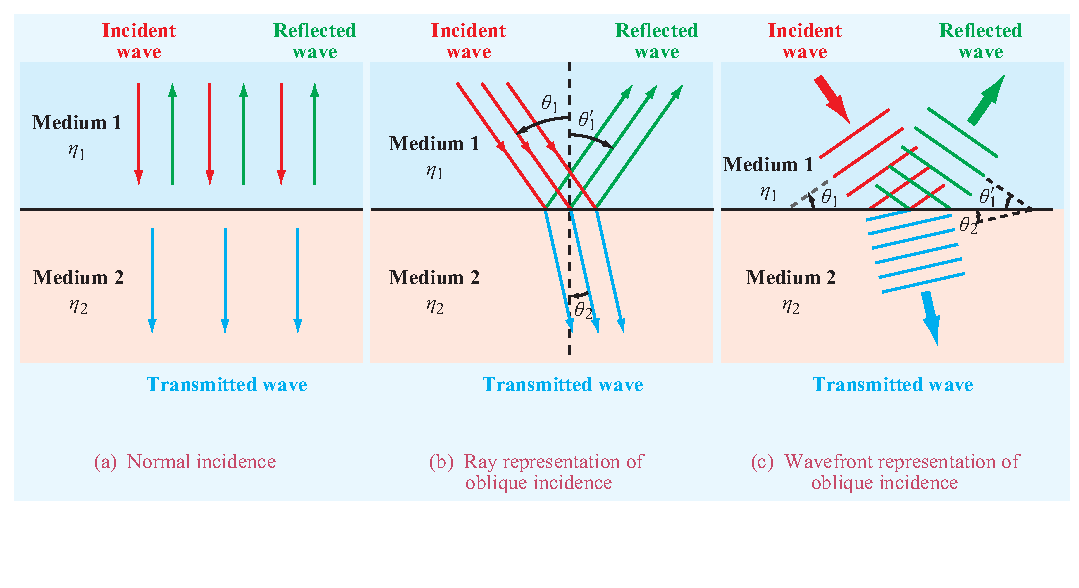
\includegraphics[width=\textwidth]{figs/em_incident_planar_basic.pdf}
\caption{(a) Normal and (b and c) oblique incidence of an EM wave to a planar boundary between two materials with different EM properties. EM waves are represented by rays in a and b, and by wavefronts in c. \emph{Rays} are lines that depict the direction of travel of waves. \emph{Wavefronts} are surfaces in which the phase of the wave is constant, and are therefore perpendicular to the direction of wave propagation. Figure reproduced from \citet{ulaby2014}, Figure 2-12.}
\label{f:reflect}
\end{center}
\end{figure}

In practice, it is often the case that a material will either be low-loss ($\varepsilon''/\varepsilon' \ll 1$) or a good conductor ($\varepsilon''/\varepsilon' \gg 1$), and simplifications to the above can be made that provide some further insight. Consider the extreme case of a nonconductive material, and note that Eq. \ref{e:alphabeta1} indicates that $\alpha \to0$ and $\beta\to k_0\sqrt{\varepsilon'}$ as $\varepsilon''\to0$, thereby recovering the model for propagation in a lossless material. For a low-loss dielectric material ($\varepsilon''/\varepsilon' \ll 1$), it is straightforward (using the binomial approximation) to show that 
	\begin{subequations}
	\label{e:alphabeta_ll1}
	\begin{align}
	\alpha &\approx \frac{k_0 \varepsilon''}{2\sqrt{\varepsilon'}} \\
	\beta &\approx k_0\sqrt{\varepsilon'} \\
	\eta_c &\approx \frac{\eta_0}{\sqrt{\varepsilon'}}
	\end{align}
	\end{subequations}
where we can see that the loss factor attenuates the signal but does not influence the phase. For a good conductor ($\varepsilon''/\varepsilon' \gg 1$), we have
	\begin{subequations}
	\label{e:alphabeta_gc1}
	\begin{align}
	\alpha &\approx k_0\sqrt{\frac{ \varepsilon''}{2}} \\
	\beta &\approx \alpha \\
	\eta_c &\approx \eta_0\frac{1+j}{\sqrt{2\varepsilon''}}
	\end{align}
	\end{subequations}
In the case of good conductor, the phase and attenuation coefficients are approximately equal and depend only on the conductivity of the material. In the extreme, $\alpha \to \beta \to \infty$ and $\eta_c\to0$ for a perfect conductor ($\sigma\to\infty$). To summarize: In a low-loss material, conductivity serves only to attenuate the signal while permittivity influences attenuation and phase. In a good conductor, permittivity plays a negligible role, and conductivity is the only important material property. These equations are summarized in Fig. \ref{f:emtable}.

\section{EM wave reflection and transmission}

In this section, we discuss reflection by and transmission through a planar boundary. In the interest of clarity, we focus first on the relatively simple case of normal incidence to a planar surface (Fig. \ref{f:reflect}a) before proceeding to the case of oblique incidence (Fig. \ref{f:reflect}b). In this discussion, we will make use of the concepts of rays and wavefronts. \emph{Rays} are lines that represent the direction of flow of EM energy carried by waves; they are parallel to the propagation (unit) vector $\hat{\mathbf{k}}$. \emph{Wavefronts} are surfaces of constant phase; they are perpendicular to $\hat{\mathbf{k}}$.

\begin{figure}[h]
\begin{center}
\begin{tabular}{c c}
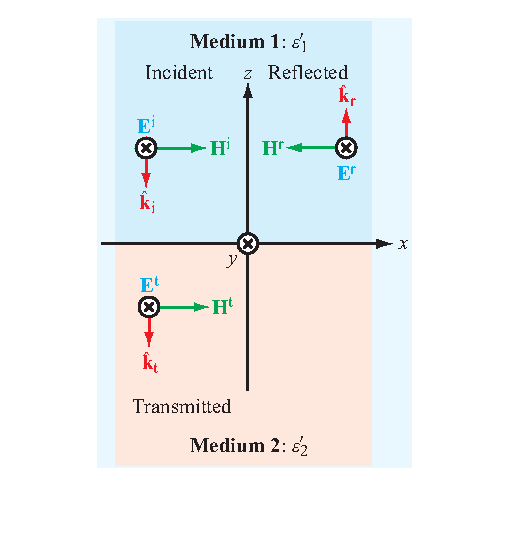
\includegraphics[height=7.5cm]{figs/em_normal_inc.pdf} & 
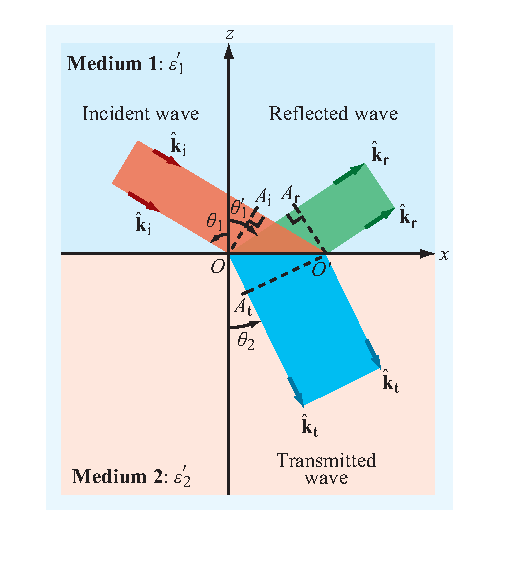
\includegraphics[height=7.5cm]{figs/em_oblique_inc.pdf}
\end{tabular}
\caption{Ray diagram for (left) normal and (right) oblique incidence. In the righthand figure, the variables containing $A$ represent the cross-sectional area of the incident, reflected, and transmitted beam. From \citet{ulaby2014}.}
\label{f:normincidence}
\end{center}
\end{figure}

\subsection{Normal incidence to a planar boundary}

We begin with the relatively simple case of normal incidence of a linearly polarized EM wave to a planar boundary between two homogenous, dielectric media. The boundary is located at $z=0$. The upper medium ($z\ge0$) has permittivity $\varepsilon_1'$ while the lower medium has permittivity $\varepsilon_2'$; both media are nonmagnetic ($\mu_1=\mu_2=\mu_0$). The incident, reflected, transmitted fields are indicated by superscripts $i$, $r$, and $t$, respectively. Similarly for propagation vectors $\hat{\mathbf{k}}$, but with subscripts $i$, $r$, and $t$. See Fig. \ref{f:normincidence} for variable definitions. 

\begin{figure}[t]
\begin{center}
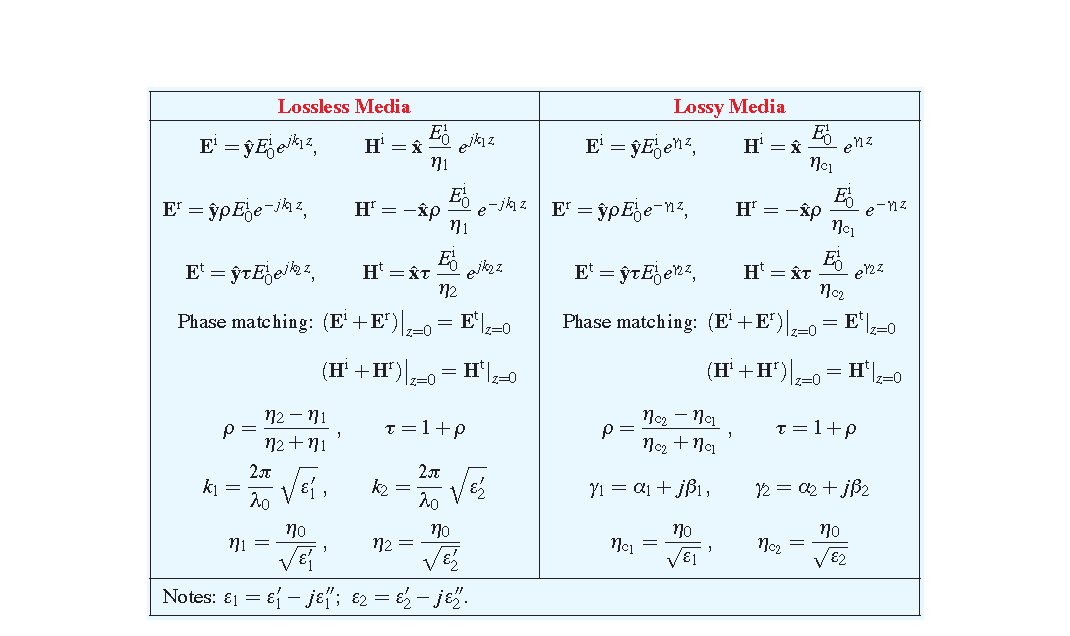
\includegraphics[width=0.85\textwidth]{figs/em_inc_table1.pdf}
\caption{A review of equations of EM fields in lossless (left) and lossy (right) media for normal incidence. Table from \citet{ulaby2014}.}
\label{f:inctable}
\end{center}
\end{figure}

The total electric and magnetic fields in each media are given as
	\begin{subequations}
	\label{e:normal_inc1}
	\begin{align}
	\mathbf{E}_1 &= \mathbf{E}^i + \mathbf{E}^r \\
	\mathbf{H}_1 &= \mathbf{H}^i + \mathbf{H}^r \\
	\mathbf{E}_2 &= \mathbf{E}^t \\
	\mathbf{H}_2 &= \mathbf{H}^t 
	\end{align}
	\end{subequations}
Suppose that the incident electric magnetic fields are known and defined such that 
	\begin{subequations}
	\label{e:normal_inc_i1}
	\begin{align}
	\mathbf{E}^i &= \hat{\mathbf{y}}E^i_0e^{\gamma_1z} \\
	\mathbf{H}^i &= \hat{\mathbf{x}}\frac{E^i_0}{\eta_{c1}}e^{\gamma_1z}
	\end{align}
	\end{subequations}
where $\gamma_1 = \alpha_1 + j\beta_1$ and $\eta_{c_1} = \eta_0/\sqrt{\varepsilon_1}$. We can then derive expressions for the reflected and transmitted fields by imposing the boundary conditions for the total electric and magnetic fields: \textbf{The tangential components of the electric and magnetic fields are continuous across a boundary between two media} (in the absence of current sources at the boundary). In the case of normal incidence, all electric and magnetic fields are tangential to the boundary. Applying the field-tangent boundary condition (sometimes called \emph{phase matching}) gives
	\begin{subequations}
	\label{e:normal_inc_rt1}
	\begin{align}
	\rho = \frac{E^r_0}{E^i_0} &= \frac{\eta_{c_2} - \eta_{c_1}}{\eta_{c_2} + \eta_{c_1}} = 
			\frac{\sqrt{\varepsilon_1} - \sqrt{\varepsilon_2}}{\sqrt{\varepsilon_1} + \sqrt{\varepsilon_2}}  \\
	\tau = \frac{E^t_0}{E^i_0} &= \frac{2\eta_{c_2}}{\eta_{c_2} + \eta_{c_1}} = \frac{2\sqrt{\varepsilon_1}}{\sqrt{\varepsilon_1} + \sqrt{\varepsilon_2}}
	\end{align}
	\end{subequations}
The terms $\rho$ and $\tau$ are commonly called the Fresnel reflection and transmission coefficients, respectively. Conservation of energy requires the Fresnel reflection and transmission coefficients to be related such that
	\begin{subequations}
	\label{e:tau_norm}
	\begin{align}
	\tau &= 1 + \rho \\ &= \sqrt{\left(1 - \rho^2\right)\frac{\eta_{c_2}}{\eta_{c_1}}}
	\end{align}
	\end{subequations}
for normal incidence. A summary of the equations in this section is given in Fig. \ref{f:inctable} for lossless (left column) and general (right column) media. 



\subsection{Oblique incidence to a planar boundary}

We now consider the case of oblique incidence, which is often encountered in remote sensing applications. In this section, we will introduce important terminology for some commonly used polarizations in remote sensing and to lay the ground work for understanding how the polarization of EM radiation can be used to glean information about the physical properties of materials that interact with the incident wave. 

\begin{figure}[t]
\begin{center}
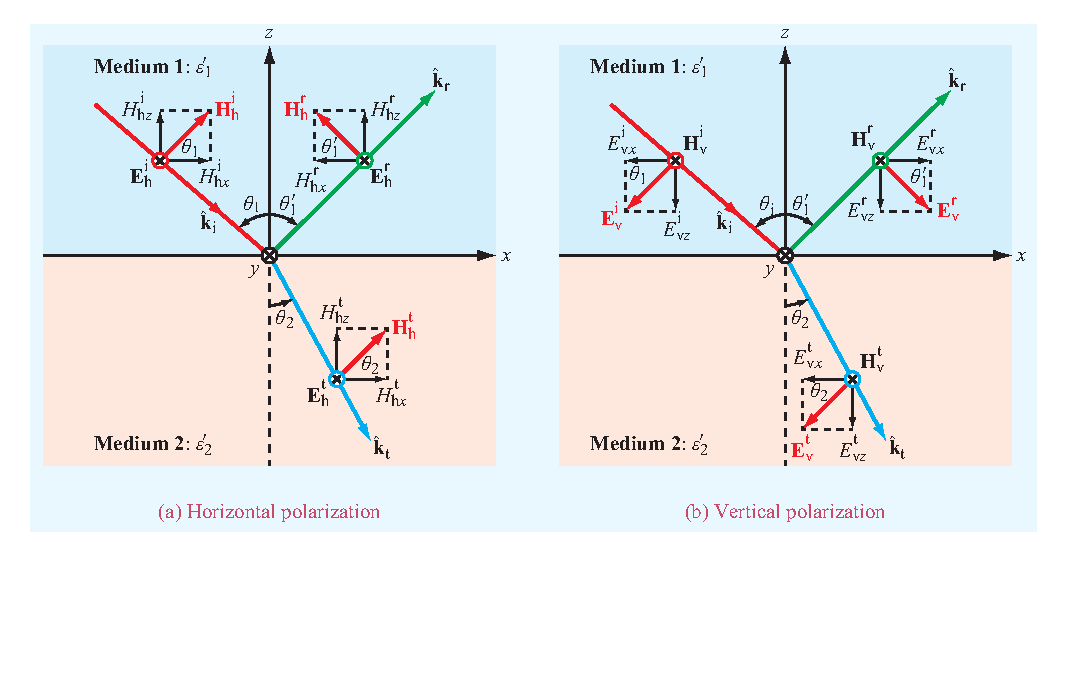
\includegraphics[width=\textwidth]{figs/em_oblique_inc2.pdf}
\caption{Schematic of the oblique incidence geometry. From \citep{ulaby2014}.}
\label{f:oblique_geo}
\end{center}
\end{figure}


Similar to the previous section, the boundary is located at $z=0$, with medium 1 on top ($z\ge0$) and medium 2 on the bottom. Medium 1 contains the incident and reflected waves. The incidence angle is $\theta_1$, the reflection angle $\theta_1'$, and the refraction angle $\theta_2$. From \emph{Snell's Laws of reflection and refraction}, we have
	\begin{subequations}
	\label{e:snells}
	\begin{align}
	\theta_1 =&\ \theta_1'   \qquad\qquad\qquad\qquad \qquad\;\;\;\; \mathrm{Snell's\ Law\ of\ reflection}  \label{e:snellreflec}\\
	\frac{\sin{\theta_2}}{\sin{\theta_1}} = &\ \frac{\mathrm{v}_{p_2}}{\mathrm{v}_{p_1}} = \frac{n_1}{n_2} = \sqrt{\frac{\varepsilon_1'}{\varepsilon_2'}} 
				\qquad\qquad\ \mathrm{Snell's\ Law\ of\ refraction} \label{e:snellrefrac}
	\end{align}
	\end{subequations}
where $\mathrm{v}_{p_i}$ is the phase velocity and $n'_i = c/\mathrm{v}_{p_i}$ the refraction index in medium $i$. From Eq. \ref{e:snellrefrac} we can see that an EM wave incident on a material with a higher permittivity ($\varepsilon_2' > \varepsilon_1'$) will refract inward ($\theta_2 < \theta_1$). Conversely, a wave incident on a material with a lower permittivity ($\varepsilon_2' < \varepsilon_1'$) will refract outward ($\theta_2 > \theta_1$). The critical angle $\theta_c$ is defined such that
	\begin{equation}
	\sin{\theta_c} = \frac{n_2}{n_1} = \sqrt{\frac{\varepsilon_2'}{\varepsilon_1'}}
	\end{equation}
and results in $\theta_2 = \pi/2$, leading to transmission along the boundary with no energy being transmitted into medium 2. If the incidence angle exceeds the critical angle, the incident wave is entirely reflected, a phenomena called total internal reflection\footnote{Because permittivity (and therefore refraction index) often scales with mass density of a material, it is common in remote sensing applications to describe materials with higher values refraction indices as more dense (and vice versa). Readers familiar with seismology will recognize the corollary between density and refraction index for fixed Lam\'e parameters.}.

Recall from the previous section the concept of \emph{phase matching}, wherein we require that the tangential components of the electric (and magnetic) field are continuous across the boundary. For normal incidence, the electric (and magnetic) fields are tangential to the boundary regardless of polarization. But for oblique incidence angles ($\theta_1 > 0$), the component of the electric field that is tangent to the surface will depend on the polarization. To help us define polarization, we will take as a reference the \emph{plane of incidence}, which is defined as the plane that contains the normal to the the boundary and the propagation unit vector of the incident wave $\hat{\mathbf{k}}_1$. A portion of the plane of incidence is shown in red in Fig. \ref{f:normincidence}. 

In remote sensing, it is common to define linearly polarized EM fields in terms of horizontal (a.k.a. perpendicular) and vertically polarized. \emph{Horizontal polarization} means that the electric field is perpendicular to the plane of incidence\footnote{Horizontal polarization is so named because it is usually perpendicular to the gravity vector.}. \emph{Vertical polarization} means that the electric field lies within the plane of incidence (and, therefore perpendicular to horizontal polarization) and perpendicular to the propagation vector\footnote{For oblique incidence, vertically polarized waves usually have a component that is along the gravity vector.}. Any arbitrary linear polarization can be decomposed into horizontal and vertical components\footnote{The distinction between horizontal and vertical polarizations only applies to nonzero incidence angles.}. Note that horizontal and vertical polarizations describe the direction of the electric field. 

%\subsection{Lossless media}

\begin{figure}[t]
\begin{center}
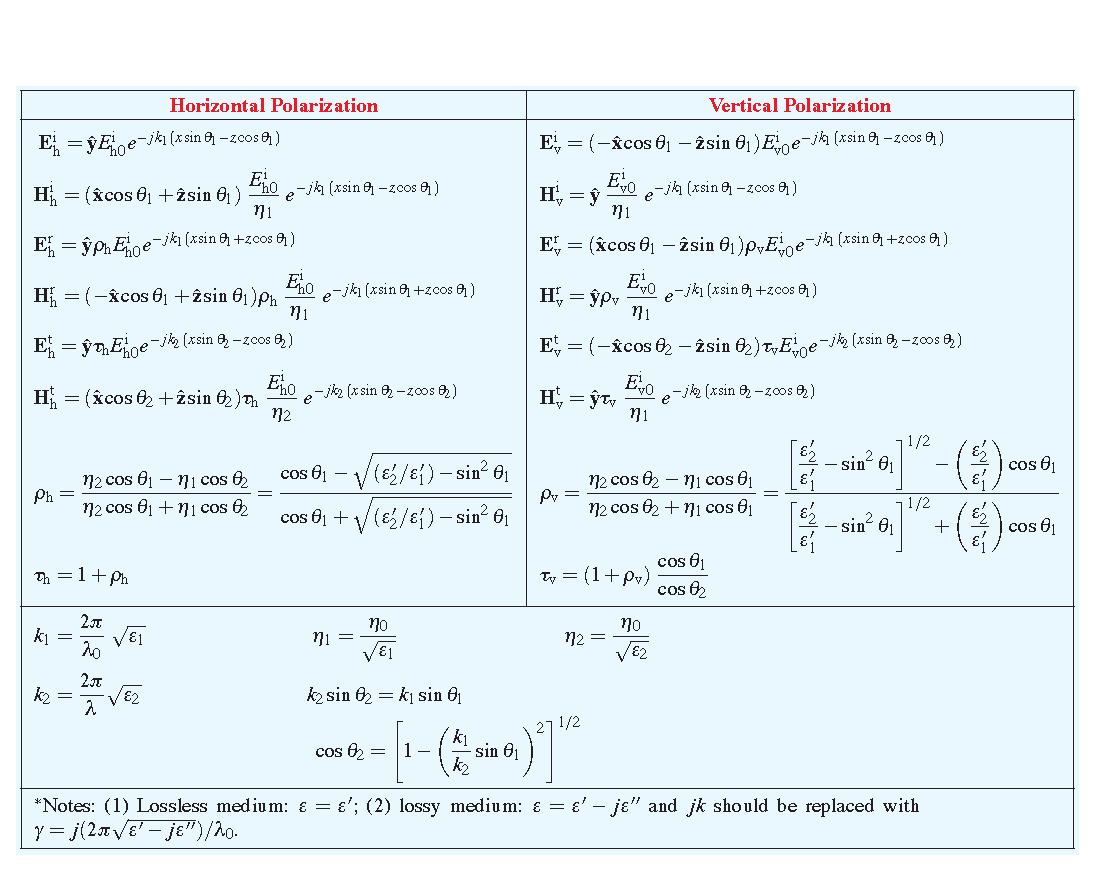
\includegraphics[width=\textwidth]{figs/em_oblique_inc3.pdf}
\caption{Equations for oblique incidence of horizontally and vertically polarized waves to lossless media. Conversion to lossy medial are discussed in the notes at the bottom. Reproduced from \citep{ulaby2014}, Table 2-4. }
\label{f:oblique_table}
\end{center}
\end{figure}


Let us consider a case where the incident wave is propagating downward, as in Fig. \ref{f:oblique_geo}. The horizontally polarized incident electric and magnetic fields are 
	\begin{subequations}
	\label{e:obliqueHi1}
	\begin{align}
	\mathbf{E}_h^i &=  E_{h0}^i e^{-\gamma_1\left(x\sin{\theta_1} - z\cos{\theta_1}\right)} \hat{\mathbf{y}} \\
	\mathbf{H}_h^i &= \frac{E_{h0}^i}{\eta_1}
				e^{-\gamma_1\left(x\sin{\theta_1} - z\cos{\theta_1}\right)}\left(\hat{\mathbf{x}}\cos{\theta_1} + \hat{\mathbf{z}}\sin{\theta_1}\right)
	\end{align}
	\end{subequations}
The horizontally polarized reflected fields are
	\begin{subequations}
	\label{e:obliqueHr1}
	\begin{align}
	\mathbf{E}_h^r &=  \rho_hE_{h0}^i e^{-\gamma_1\left(x\sin{\theta_1} + z\cos{\theta_1}\right)} \hat{\mathbf{y}} \\
	\mathbf{H}_h^r &= \rho_h\frac{E_{h0}^i}{\eta_1}
				e^{-\gamma_1\left(x\sin{\theta_1} + z\cos{\theta_1}\right)}\left(-\hat{\mathbf{x}}\cos{\theta_1} + \hat{\mathbf{z}}\sin{\theta_1}\right)
	\end{align}
	\end{subequations}
and the horizontally polarized transmitted fields are
	\begin{subequations}
	\label{e:obliqueHt1}
	\begin{align}
	\mathbf{E}_h^t &= \tau_h E_{h0}^i e^{-\gamma_2\left(x\sin{\theta_2} - z\cos{\theta_2}\right)}\hat{\mathbf{y}} \\
	\mathbf{H}_h^t &= \tau_h\frac{E_{h0}^i}{\eta_1}e^{-\gamma_2\left(x\sin{\theta_2} - z\cos{\theta_2}\right)}
					\left(\hat{\mathbf{x}}\cos{\theta_2} + \hat{\mathbf{z}}\sin{\theta_2}\right)
	\end{align}
	\end{subequations} 
Imposing continuity of the tangential component of the electric field across the boundary leads definitions of the Fresnel reflection and transmission coefficients for horizontal polarization
	\begin{subequations}
	\label{e:oblique_coefs1}
	\begin{align}
	\rho_h &= \frac{E_{h0}^r}{E_{h0}^i} = \frac{\eta_2\cos{\theta_1} - \eta_1\cos{\theta_2}}{\eta_2\cos{\theta_1} + \eta_1\cos{\theta_2}} \\
	\tau_h &= \frac{E_{h0}^t}{E_{h0}^i} = \frac{2\eta_2\cos{\theta_1}}{\eta_2\cos{\theta_1} + \eta_1\cos{\theta_2}}
	\end{align}
	\end{subequations} 
As with normal incidence, the reflection and transmission coefficients are related as
	\begin{equation}
	\tau_h = 1 + \rho_h
	\end{equation}
Applying Snell's Law, we can rewrite the Fresnel reflection coefficient for horizontal polarization as
	\begin{equation}
	\rho_h = \frac{\cos{\theta_1} - \sqrt{\left(\varepsilon_2/\varepsilon_1\right) - \sin^2{\theta_1}}}{
			\cos{\theta_1} + \sqrt{\left(\varepsilon_2/\varepsilon_1\right) - \sin^2{\theta_1}}}
	\end{equation}
For lossless media, this expression can be written in terms of the real component of the index of refraction because $\varepsilon'_2/\varepsilon'_1 = (n_2/n_1)^2$. 

Because the electric and magnetic fields are orthogonal, vertical polarization can be readily obtained from the horizontal polarized case by replacing $\mathbf{E}$ with $\mathbf{H}$ and $\mathbf{H}$ with $-\mathbf{E}$. The resulting Fresnel reflection coefficient for vertically polarized EM waves is
	\begin{subequations}
	\label{e:oblique_fresnel_vr1}
	\begin{align}
	\rho_v &= \frac{E_{v0}^r}{E_{v0}^i} = \frac{\eta_2\cos{\theta_2} - \eta_1\cos{\theta_1}}{\eta_2\cos{\theta_2} + \eta_1\cos{\theta_1}} \\
		&= \frac{\displaystyle - \frac{\varepsilon_2}{\varepsilon_1}\cos{\theta_1} + \sqrt{\frac{\varepsilon_2}{\varepsilon_1} - \sin^2{\theta_1}}}
			{\displaystyle \frac{\varepsilon_2}{\varepsilon_1}\cos{\theta_1} + \sqrt{\frac{\varepsilon_2}{\varepsilon_1} - \sin^2{\theta_1}}}
	\end{align}
	\end{subequations} 
and the Fresnel reflection coefficient is
	\begin{equation}
	\tau_v = \frac{E_{v0}^t}{E_{v0}^i} = \left(1 + \rho_v\right)\frac{\cos{\theta_1}}{\cos{\theta_2}}
	\end{equation}
These results are summarized in Fig. \ref{f:oblique_table}. 

\section*{Notation}
Throughout these notes, bolded variables indicate vectors while normal fonts indicate scalars. Hats signify unit vectors. 
\begin{longtable}{l l c}
	$a_i$ & magnitude of the electric field in the $i$-direction & V/m \\
	$c$ & speed of light in a vacuum & m/s \\
	$\mathbf{E}$ & electric field intensity & V/m \\
	$\mathbf{H}$ & magnetic field intensity & A/m \\
	$j$ & imaginary unit ($j^2 = -1$) & - \\
	$k$ & angular wavenumber ($ck=\omega$) & rad/m \\
	$n$ & complex index of refraction ($n=n'+-jn''=\sqrt{\varepsilon}$) & - \\
	$S_i$ & Stokes parameters ($i=0,1,2,3$) & V$^2$/m$^2$ \\
	$\mathrm{v}_p$ & phase velocity & m/s \\
	$\mathrm{v}_g$ & group velocity & m/s \\
	$\gamma$ & propagation constant & rad/m \\
	$\delta_i$ & relative phase in the $i$-direction & rad \\
	$\delta$ & differential phase (e.g., $\delta_x - \delta_y$) & rad \\
	$\delta_s$ & skin depth & m\\
	$\delta_p$ & penetration depth & m \\
	$\varepsilon_0$ & permittivity of free space & F/m \\
	$ \varepsilon' $ & relative (to free space) permittivity & - \\
	$ \varepsilon'' $ & relative dielectric loss factor & - \\
	$ \varepsilon$ & relative dielectric constant ($\varepsilon = \varepsilon' + j\varepsilon''$) & - \\ 
	$\eta$ & intrinsic impedance & V/A \\
	$\eta_c$ & intrinsic impedance of a conductive (lossy) medium & V/A \\
	$\eta_0$ & intrinsic impedance of free space & V/A \\
	$\lambda$ & wavelength & m \\
	$\mu$ & magnetic permeability & H/m \\
	$\rho$ & Fresnel reflection coefficient & - \\
	$\rho_v$ & charge density & C/m \\
	$\sigma$ & conductivity & S/m \\
	$\tau$ & Fresnel transmission coefficient & - \\
	$\phi$ & absolute phase & rad \\
	$\chi$ & polarization ellipticity angle & rad \\
	$\psi$ & polarization ellipse orientation angle & rad \\
	$\omega$ & angular frequency & rad/s \\
\end{longtable}


\section*{Glossary}
\renewcommand\labelitemi{{\boldmath$\cdot$}}
\begin{itemize}
	\item dielectric loss factor: $\varepsilon'' = \sigma/(\omega\varepsilon_0)$ describes the attenuation of an EM wave with angular frequency $\omega$ interacting with a material with conductivity $\sigma$
	\item free space: A perfect vacuum
	\item horizontal polarization: electric field is perpendicular to the plane of incidence
	\item lossy (lossless) materials: A conductive (nonconductive) material that attenuates (or not) an EM signal
	\item penetration depth: depth at which the power of the EM signal decreases by a factor of $1/e$
	\item permittivity: measure of material's ability to store electrical energy in an electric field
	\item permeability: measure of material's ability to support the development of a magnetic field
	\item phase matching: boundary condition stating that the tangential components of the total electric and magnetic fields are continuous across a boundary between two media
	\item plane of incidence: plane that contains the normal to a boundary between two media and the propagation vector of the incident wave
	\item polarization: (of a uniform plane wave) describes the path traced by the tip of the $\mathbf{E}$ vector over time at a given point in space 
	\item ray: line representing the direction of flow of EM energy carried by waves
	\item skin depth: depth at which the magnitude of the EM signal decreases by a factor of $1/e$
	\item Snell's law of reflection: angle of reflection equals the angle of incidence
	\item Snell's law of refraction: ratio of the sins of the refraction and incidence angle is equal to the ratio of the phase velocities (or, equivalently, the real components of the refraction indices) in each medium
	\item spectroscopy: interaction of matter and EM radiation as a function of frequency or wavelength
	\item vertical polarization: electric field lies within the plane of incidence and is perpendicular to the propagation vector
	\item wavefront: surface of constant phase of a wave
\end{itemize}

\bibliography{/Users/brentminchew/Dropbox/Teaching/remote_sensing/principles/2018/notes/em.bib}
\bibliographystyle{abbrvnat}
\end{document}  
